%me=0 student solutions (ps file), me=1 - my solutions (sol file), me=2 - assignment (hw file)
\def\me{0}
\def\num{1}  %homework number
\def\due{Tuesday, September 15}  %due date
\def\course{CSCI-GA.1170-001/002 Fundamental Algorithms} %course name, changed only once
\def\name{GOWTHAM GOLI (N17656180)}   %student changes (instructor keeps!)
%
\iffalse
INSTRUCTIONS: replace # by the homework number.
(if this is not ps#.tex, use the right file name)

  Clip out the ********* INSERT HERE ********* bits below and insert
appropriate TeX code.  Once you are done with your file, run

  ``latex ps#.tex''

from a UNIX prompt.  If your LaTeX code is clean, the latex will exit
back to a prompt.  To see intermediate results, type

  ``xdvi ps#.dvi'' (from UNIX prompt)
  ``yap ps#.dvi'' (if using MikTex in Windows)

after compilation. Once you are done, run

  ``dvips ps#.dvi''

which should print your file to the nearest printer.  There will be
residual files called ps#.log, ps#.aux, and ps#.dvi.  All these can be
deleted, but do not delete ps1.tex. To generate postscript file ps#.ps,
run

  ``dvips -o ps#.ps ps#.dvi''

I assume you know how to print .ps files (``lpr -Pprinter ps#.ps'')
\fi
%
\documentclass[11pt]{article}
\usepackage{amsfonts}
\usepackage{latexsym}
\usepackage[lined,boxed,linesnumbered]{algorithm2e}
\usepackage{amsmath}
\usepackage{amssymb}
\usepackage{amsthm}
\usepackage{epsfig}
\usepackage{psfrag}
\usepackage{color}
\usepackage{tikz}
\usetikzlibrary{trees}
\usepackage{mathtools}
\usepackage{float}
\setlength{\oddsidemargin}{.0in}
\setlength{\evensidemargin}{.0in}
\setlength{\textwidth}{6.5in}
\setlength{\topmargin}{-0.4in}
\setlength{\textheight}{8.5in}

\newcommand{\handout}[5]{
   \renewcommand{\thepage}{#1, Page \arabic{page}}
   \noindent
   \begin{center}
   \framebox{
      \vbox{
    \hbox to 5.78in { {\bf \course} \hfill #2 }
       \vspace{4mm}
       \hbox to 5.78in { {\Large \hfill #5  \hfill} }
       \vspace{2mm}
       \hbox to 5.78in { {\it #3 \hfill #4} }
      }
   }
   \end{center}
   \vspace*{4mm}
}

\newcounter{pppp}
\newcommand{\prob}{\arabic{pppp}}  %problem number
\newcommand{\increase}{\addtocounter{pppp}{1}}  %problem number
\newcommand{\comment}[1]{}

%first argument desription, second number of points
\newcommand{\newproblem}[2]{
\ifnum\me=0
\ifnum\prob>0 \newpage \fi
\increase
\setcounter{page}{1}
\handout{\name, Homework \num, Problem \arabic{pppp}}{\today}{Name: \name}{Due:
\due}{Solutions to Problem \prob\ of Homework \num\ (#2)}
\else
\increase
\section*{Problem \num-\prob~(#1) \hfill {#2}}
\fi
}

%\newcommand{\newproblem}[2]{\increase
%\section*{Problem \num-\prob~(#1) \hfill {#2}}
%}

\def\squarebox#1{\hbox to #1{\hfill\vbox to #1{\vfill}}}
\def\qed{\hspace*{\fill}
        \vbox{\hrule\hbox{\vrule\squarebox{.667em}\vrule}\hrule}}
\newenvironment{solution}{\begin{trivlist}\item[]{\bf Solution:}}
                      {\qed \end{trivlist}}
\newenvironment{solsketch}{\begin{trivlist}\item[]{\bf Solution Sketch:}}
                      {\qed \end{trivlist}}
\newenvironment{code}{\begin{tabbing}
12345\=12345\=12345\=12345\=12345\=12345\=12345\=12345\= \kill }
{\end{tabbing}}



\newcommand{\hint}[1]{({\bf Hint}: {#1})}
%Put more macros here, as needed.
\newcommand{\room}{\medskip\ni}
\newcommand{\brak}[1]{\langle #1 \rangle}
\newcommand{\bit}[1]{\{0,1\}^{#1}}
\newcommand{\zo}{\{0,1\}}
\newcommand{\C}{{\cal C}}

\newcommand{\nin}{\not\in}
\newcommand{\set}[1]{\{#1\}}
\renewcommand{\ni}{\noindent}
\renewcommand{\gets}{\leftarrow}
\renewcommand{\to}{\rightarrow}
\newcommand{\assign}{:=}

\newcommand{\AND}{\wedge}
\newcommand{\OR}{\vee}


\begin{document}

\ifnum\me=0
%\handout{PS\num}{\today}{Name: **** INSERT YOU NAME HERE ****}{Due:
%\due}{Solutions to Problem Set \num}
%
%I collaborated with *********** INSERT COLLABORATORS HERE (INDICATING
%SPECIFIC PROBLEMS) *************.
\fi
\ifnum\me=1
\handout{PS\num}{\today}{Name: Yevgeniy Dodis}{Due: \due}{Solution
{\em Sketches} to Problem Set \num}
\fi
\ifnum\me=2
\handout{PS\num}{\today}{Lecturer: Yevgeniy Dodis}{Due: \due}{Problem
Set \num}
\fi


\newproblem{Insertion Sort Using a Linked List}{10 points}

Consider the problem of implementing insertion sort using a
doubly-linked list instead of array. Namely, each element $a$ of the
linked list has fields $a.previous$, $a.next$ and $a.value$. You are
giving a stating element $s$ of the linked list (so that
$s.previous=nil$, $s.value = A[1]$, $s.next.value = A[2]$, etc.)

\begin{itemize}

\item[(a)](8 points) Give a pseudocode implementation of this algorithm, and
analyze its running time in the $\Theta(f(n))$ notation. Explain how
we do not have to ``bump'' elements in order to create room for the
next inserted elements. Is this saving asymptotically significant?

\ifnum\me<2
\begin{solution} 

As explained in the class, Insertion Sort, In each iteration takes one input from the array (or in this case a doubly-linked list) and correspondingly produces a sorted output array (or a sorted doubly-linked list). 

In each iteration, the chosen element or the key from the list is placed in the appropriated position in the sorted list to it's left. This is repeated until the entire list is sorted

\comment{
\begin{figure}[h]
	\centering
	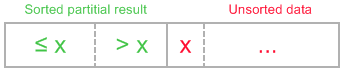
\includegraphics[width=0.5\columnwidth]{insertion-sort.png}
	\caption{Insertion Sort}
	\label{1}
\end{figure} 
}

{\bf Psuedo Code}

In the following Psuedo code, 
\begin{itemize}
\item \textit{keyNode} represents the node in the doubly-linked list that is to be inserted in the appropriate position in the sorted list to it's left
\item \textit{SortedListTail} represents the tail node of the sorted list to the left of \textit{keyNode}
\item \textit{s} represents the head or the starting element of the doubly-linked list
\end{itemize}


\IncMargin{1em}
\begin{algorithm}[H]
\TitleOfAlgo{InsertionSort(s)}
keyNode $\leftarrow$ s.next\;
SortedListTail $\leftarrow$ keyNode.prev\;
\While{keyNode is not \textbf{NULL}}{
	nextkeyNode $\leftarrow$ keyNode.next\;
	Node $\leftarrow$ SortedListTail\;
	\While{Node is not \textbf{NULL} and Node $>$ keyNode}{
		Node = Node.prev\;
	}
	\If{Node is \textbf{NULL}}{
		SortedListTail.next = nextkeyNode\;
		nextkeyNode.prev = SortedListTail\;
		keyNode.prev = \textbf{NULL}\;
		keyNode.next = s\;
		s.prev = keyNode\;
		s = keyNode\;
	}
	\Else{
	SortedListTail.next = nextkeyNode\;
	nextkeyNode.prev = sortedListTail\;
	keyNode.next = Node.next\;
	Node.next.prev = keyNode\;
	Node.next = keyNode\;
	keyNode.prev = Node\;
	
	}
	keyNode $\leftarrow$ nextkeyNode\;
	sortedListTail $\leftarrow$ keyNode.prev\;

}
\SetAlgoLined

\caption{Insertion Sort on a doubly-linked list in $O(n^2)$ time}
\end{algorithm}

{\bf Time Complexity}

In the worst case scenario, the key node always gets inserted at the beginning or the head of the partially sorted list, thus having to traverse the entire sorted list starting from it's tail (i.e the previous node of key node). Thus the total number of computations atmost will be $1+2+3+\ldots+n-1 = (n-1)(n-2)/2$. i.e $T(n) = O(n^2)$

{\bf Is using doubly-linked list asymptotically significant?}

In the case of doubly-lined list (as opposed to arrays), we do not need to swap the key element each time that we find an element greater to the key in the partially sorted list. Instead, we keep traversing the  sorted list until we find a suitable position for the key node and insert it there accordingly, updating the previous and next pointers of the involved nodes as seen in the pseduo code. Thus we do not have to bump each element as we did previously in case of arrays.\\
Each bump (or swapping two elements in the array) takes only $O(1)$ time. Hence this saving is not asymptotically significant and the time complexity still remains to be $O(n^2)$

\end{solution}
\fi

\item[(b)] (2 points) Can we speed up the time of the implementation to
$O(n \log n)$ by utilizing binary search?

\ifnum\me<2
\begin{solution}
To implement binary search list in a doubly-linked list we proceed as follows
\begin{itemize}
\item Traverse till the middle node. If it matches then return it
\item If the node is bigger, discard the right half of the list and use binary search in the remaining left half of the list
\item If the node is smaller, discard the left half of the list and use binary search in the remaining right half of the list
\item Keep repeating these steps until we find the required node
\end{itemize}

The first step requires $n/2$ steps. From there on we traverse to middle element of the remaining half list which takes $n/4$ steps, then traverse to middle element of the quarter of the list which takes $n/8$ steps.\\
 Thus, the total number of steps will be $n+n/2+n/4+n/8+\ldots = n$. Therefore, binary search in  a doubly-linked list still takes $O(n)$ time which is same as that of a linear search. Hence, there will not be any difference and the time complexity still remains to be $O(n^2)$  
\end{solution}
\fi

\end{itemize}


\newproblem{Multiplying Binary Integers}{10 Points}

You are given two $n$-bit binary integers $a$ and $b$. These integers
are stored in two arrays $A[0,\ldots, n-1]$ and $B[0,\ldots, n-1]$
{\em in reverse}, so that $a = \sum_{i=0}^{n-1} A[i]\cdot 2^i$ and $b
= \sum_{i=0}^{n-1 } B[i]\cdot 2^i$. For example, if $n=6$ and
$a=000111$ (7 in decimal) and $b=100011$ (35 in decimal), then
$A[0]=A[1]=A[2]=1$, $A[3]=A[4]=A[5]=0$, $B[0]=B[1]=B[5]=1$,
$B[2]=B[3]=B[4]=0$. Your goal is to produce an array $C[0,\ldots
2n-1]$ which stores the product $c$ of $a$ and $b$. For example,
$000111\cdot 100011 = 7 \cdot 35 = 245 = 000011110101$, meaning
that $C[0\ldots 11] = 101011110000$.

\begin{itemize}

\item[(a)] (2 points) Prove that $c=\sum_{(i: B[i]=1)} (a\cdot 2^i)$.

\ifnum\me<2
\begin{solution}
Given
\begin{align*}
a &= \sum_{i=0}^{n-1}A[i].2^i \\
b &= \sum_{i=0}^{n-1}B[i].2^i\\
c &= a.b\\
\implies c &= a.(\sum_{i=0}^{n-1}B[i].2^i)\\
\end{align*}

We know that the only possible values of $B[i]$ are $0$ and $1$

\begin{align*}
\implies c &= a.(\sum_{(i:B[i]=1)}B[i].2^i + \sum_{(i:B[i]=0)}B[i].2^i)\\
&= a.(\sum_{(i:B[i]=1)}1.2^i + \sum_{(i:B[i]=0)}0.2^i)\\
&= a.(\sum_{(i:B[i]=1)}2^i)\\
&= \sum_{(i:B[i]=1)}(a.2^i)\\
\end{align*}
\end{solution}
\fi

\item[(b)] (4 points) Write an $O(n+i)$ time procedure {\sc Shift}$(A,n,i)$ to compute
the $(n+i)$-bit product $a\cdot 2^i$.

\ifnum\me<2
\begin{solution}
Multiplying any n-bit integer $a$ by $2^i$ is equivalent to left shifting the bit integer by $i$ places resulting in a new (n+i)-bit integer. The pseudo code for shift is as follows\\

{\bf Psuedo Code}

\IncMargin{1em}
\begin{algorithm}[H]
\TitleOfAlgo{SHIFT(A, n, i)}
ShiftedArray $\leftarrow$ malloc(n+i)			//Allocate new array of length $n+i$\\
\For{k = n+i to i}{
	ShiftedArray[k] = A[k-i]
}
\For{k = i-1 to 0}{
	ShiftedArray[k] = 0
}
$return$ ShiftedArray
\SetAlgoLined

\caption{Left shift array $A$ of length $n$ by $i$ places}
\end{algorithm}
 
\end{solution}
\fi

{\bf Time Complexity}

As seen in the Psuedo code, we are just traversing the entire $ShiftedArray$ using the two $for$ loops. Therefore, $T(n) = O(n+i)$

\item[(c)] (4 points) Assume you are given $O(n)$ procedure {\sc Add}$(X,m,Y,k)$ which adds
an $m$-bit $X$ to $k$-bit $Y$, where $m,k\le 2n$. Using this
procedure, and your work in parts (a) and (b), write the pseudocode to
produce the desired product array $C$. Analyze the running
time of your procedure in the $\Theta(f(n))$ notation, for appropriate
function $f(n)$.

\ifnum\me<2
\begin{solution}
From part(a), we know that $c = c = \sum_{(i:B[i]=1)}(a.2^i)$. Now, the idea is to calculate each term of the summation using the $SHIFT(A,n,i)$ method from part(b) and then add all these terms using $ADD(X,m,Y,k)$\\

{\bf Psuedo Code}

\IncMargin{1em}
\begin{algorithm}[H]
\TitleOfAlgo{MUTIPLY(A,B)}
C $\leftarrow$ 0\;
numTerms $\leftarrow$ 0\;
\For{i = 0 to n-1}{
	\If{B[i] is 1}{
		ShiftedArray[numTerms] = SHIFT(A,n,i)\;
		numTerms++\;
	}
}

\For{i = 0 to numTerms}{
	C = ADD(C, C.length, ShiftedArray[i], ShiftedArray[i].length)
}

return C

\SetAlgoLined
\caption{Multiply two n-bit integers $a$ and $b$ using $SHIFT$ and $ADD$}
\end{algorithm}

{\bf Time Complexity}

In the worst case scenario, all the bits of both the arrays or either of the arrays is $1$. Therefore,\\
In the \textit{Shift} step, time taken to shift each of the $n$ terms of the summation by $i$ places will be\\ $\sum_{i=1}^{n}(n+i) = O(n^2)$.

In the \textit{Add} step, time taken to add two consecutive bit integers (derived from \textit{Shift} step) is $O(n)$ and the iteration is repeated until all the $n$ terms are added, Hence total time is $O(n^2)$.

Therefore, the time complexity of Shift and Add multiplication is $O(n^2)$.

\end{solution}
\fi

\end{itemize}



\newproblem{Polynomial Evaluation}{ 16 (+4) Points}

A degree-$n$ polynomial $P(x)$ is a function
$$P(x) = a_0 + a_1x + \ldots + a_{n-1}x^{n-1} + a_n x^n = \sum_{i=0}^n a_i
x^i$$

\begin{itemize}

\item[(a)] (2 points) Express the value $P(x)$ as
$$P(x) = a_0 + a_1x + \ldots + a_{n-2} x^{n-2} + b_{n-1} x^{n-1} =
\sum_{i=0}^{n-1} b_i x^i$$
where $b_0=a_0,\ldots, b_{n-2} = a_{n-2}$. What is $b_{n-1}$ as a
function of the $a_i$'s and $x$?

\ifnum\me<2
\begin{solution}
\begin{align*}
Given,
P(x) &= a_0+a_1x+\ldots+a_{n-1}x^{n-1}+a_nx^n = \sum_{i=0}^{n}a_ix^i\\
\implies P(x) &= a_0+a_1x+\ldots+a_{n-2}x^{n-2}+x^{n-1}(a_{n-1}+ a_nx)\\
\end{align*}
Let   $b_0 = a_0, \ldots, b_{n-2} = a_{n-2}$ and $b_{n-1} = a_{n-1}+ a_nx$
\begin{align*}
\implies P(x) &= b_0+b_1x+\ldots+b_{n-2}x^{n-2}+b{n-1}x^{n-1}\\
&= \sum_{i=0}^{n-1}b_ix^i
\end{align*}
where $ b_k = a_k, \forall \,\, k = 0,\ldots, n-2$ and $b_{n-1} = a_{n-1}+ a_nx$

\end{solution}
\fi

\item[(b)] (5 points) Using part (a) above write a recursive procedure
$\mathsf{Eval}(A,n,x)$ to evaluate the polynomial $P(x)$ whose
coefficients are given in the array $A[0\ldots n]$ (i.e., $A[0]=a_0$,
etc.). Make sure you do not forget the base case $n=0$.

\ifnum\me<2
\begin{solution} From part(a)
\begin{align*}
P(x) = \sum_{i=0}^{n-1}b_ix^i\\
\end{align*}
where $b_k = a_k, \forall \,\ k = 0,\ldots, n-2$ and $b_{n-1} = a_{n-1}+ a_nx$\\

Similarly, we can reduce $P(x)$ to as follows
\begin{align*}
P(x) = \sum_{i=0}^{n-2}c_ix^i\\
\end{align*}
where $c_k = b_k, \forall \,\ k = 0,\ldots, n-3$ and $c_{n-2} = b_{n-2}+ b_{n-1}x$

$\implies c_k = a_k, \forall \,\ k = 0,\ldots, n-3$ and $c_{n-2} = a_{n-2}+ b_{n-1}x \,\,\,\,(\because b_k = a_k, \forall \,\ k = 0,\ldots, n-2)$ \\

Similarly, further reducing $P(x)$ we get
\begin{align*}
P(x) = \sum_{i=0}^{n-3}d_ix^i
\end{align*}
where $d_k = c_k, \forall \,\ k = 0,\ldots, n-4$ and $d_{n-3} = c_{n-3}+ c_{n-2}x$

$\implies d_k = a_k, \forall \,\ k = 0,\ldots, n-4$ and $d_{n-3} = a_{n-3}+ c_{n-2}x \,\,\,\,(\because c_k = a_k, \forall \,\ k = 0,\ldots, n-3)$ \\

On further reduction,

$\vdots$ \\
$\vdots$\\

\begin{align*}
P(x) = \sum_{i=0}^{1}z_ix^i\\
\end{align*}
where $z_k = a_k$ for $k=0$ and $z_1 = a_1+ y_2x$
$\implies P(x) = a_0 + z_1x$

Define new variables $p_1, p_2, \ldots , p_n$ such that
\begin{align*}
p_n &= b_n  = a_n\\
p_{n-1}&= b_{n-1} \\
p_{n-2} &= c_{n-2}\\
p_{n-3} &= d_{n-3}\\
\vdots\\
p_2 &= y_2\\
p_1 &= z_{1}
\end{align*}

Now substituting $p_1, p_2, \ldots, p_n$ into the above obtained results we get,  

\begin{equation*}
\begin{aligned}
p_n &= a_n\\
p_{n-1} &= a_{n-1} +p_nx\\
p_{n-2} &= a_{n-2} +p_{n-1}x\\
\vdots\\
p_1 &= a_1 + p_2x\\
P(x) &= a_0 + p_1x\\
\end{aligned}
\end{equation*}

$\therefore$ From the above equations, it can be easily seen that the recurrence relation is as follows
\begin{equation*}
\begin{aligned}
P(x) &= a_0 + p_1x\\
p_i &= a_i + p_{i+1}x,  \,\,\,\,\,\,\,\,\,\,\,\,\,     \forall i = 1,\ldots,n-1\\
p_n &= a_n\\
\end{aligned}
\end{equation*}


{\bf Psuedo Code}

$Eval(A,0,x)$ is the starting point of recursion

\IncMargin{1em}
\begin{algorithm}[H]
\TitleOfAlgo{Eval(A, k, x)}

\If{ k is n}{
	return $a_n$
}
\Else{
	return $a_k$ + Eval$(A, k+1, x)$ 
}

\SetAlgoLined
\caption{Evaluate polynomial $P(x)$ using recursion}
\end{algorithm}

\end{solution}
\fi

\item[(c)] (3 points) Let $T(n)$ be the running time of your implementation
of $\mathsf{Eval}$. Write a recurrence equation for $T(n)$ and solve
it in the $\Theta(\cdot)$ notation.

\ifnum\me<2
\begin{solution}
The recursion tree looks like follows 

\begin{figure}[H]
\centering
\begin{tikzpicture}[level distance=1.5cm,
  level 1/.style={sibling distance=3cm},
  level 2/.style={sibling distance=1.5cm}]
  
  \node {Eval(A, 0, x)}
    child {node {$a_0$}}
    child {node {Eval(A, 1, x)}
    child {node {$a_1$}}
      child {node {Eval(A, 2, x)}
      	child{node{$a_2$}}
      	child{node{$\vdots$}}
      }
    };
\end{tikzpicture}
\end{figure}

The height of the tree is $n$ as the final call of the recursion is $Eval(A, n ,x)$. At each level of the tree, total number of executions done is of $O(1)$. 

\begin{equation}
  \begin{aligned}
        \therefore T(n) &= T(n-1) + O(1)\\
                &= T(n-2) + O(1) + O(1)\\
                &= \underbrace{O(1) + O(1) + \ldots + O(1)}_\text{n terms}\\
                &= nO(1)\\ 
                &= O(n)\\
  \end{aligned}
\end{equation}

\end{solution}
\fi

\item[(d)] (6 points) Assuming $n$ is a power of $2$, try to express $P(x)$ as
$P(x) = P_0(x) + x^{n/2}P_1(x)$, where $P_0(x)$ and $P_1(x)$ are both
polynomials of degree $n/2$. Assuming the computation of $x^{n/2}$
takes $O(n)$ times, describe (in words or pseudocode) a recursive
procedure $\mathsf{Eval}_2$ to compute $P(x)$ using two recursive
calls to $\mathsf{Eval}_2$. Write a recurrence relation for the
running time of $\mathsf{Eval}_2$ and solve it. How does your solution
compare to your solution in part (c)?

\ifnum\me<2
\begin{solution}
Given,
\begin{align*}
P(x) &= a_0 + a_1x+ \ldots + a_{n-1}x^{n-1}+ a_nx^n\\
&= a_0+a_1x+\ldots+ a_{n/2-1}x^{n/2-1}+a_{n/2}x^{n/2}+\ldots+a_{n-1}x^{n-1}+a_nx^n\\
&= ( a_0+a_1x+\ldots+ a_{n/2-1}x^{n/2-1})+ x^{n/2}(a_{n/2}+ \ldots+ a_{n-1}x^{n/2-1}+a_nx^{n/2})\\
&= ( a_0+a_1x+\ldots+ a_{n/2-1}x^{n/2-1} + a^{'}_{n/2}x^{n/2})+ x^{n/2}(a_{n/2}+ \ldots+ a_{n-1}x^{n/2-1}+a_nx^{n/2})\\
&= P_0(x)+x^{n/2}P_1(x)\\
\end{align*}
\newline
where 

$P_0(x) = a_0+a_1x+\ldots+ a_{n/2-1}x^{n/2-1} + a^{'}_{n/2}x^{n/2},\,\,\,\,\,\,(a^{'}_{n/2} = 0)$

$P_1(x) = a_{n/2}+ a_{n/2+1}x\ldots+ a_{n-1}x^{n/2-1}+a_nx^{n/2}$

Therefore, $P(x)$ can be evaluated by evaluating $P_0(x)$, $P_1(x)$ and $x^{n/2}$ which can be done through recursion as seen in the following Psuedo Code\\

{\bf Psuedo Code}

\IncMargin{1em}
\begin{algorithm}[H]
\TitleOfAlgo{Eval$_2$(P,n,x)}
\If{n is 1}{
	\textbf{return} $a_0+a_1x$
}
\Else{
	\textbf{return}	$Eval_2(P_0,n/2,x) + x^{n/2}.Eval_2(P_1,n/2,x)$
}
\SetAlgoLined
\caption{Algorithm to evaluate the value of $P(x)$ using divide and conquer}
\end{algorithm}

{\bf Time Complexity}

$P(x)$ can be evaluated using divide and conquer as seen above.\\
In the divide step, we split $P(x)$ into two polynomials, $P_0(x)$ and $P_1(x)$ of degree $n/2$. \\
In the conquer step, we multiply $P_1(x)$ with $x^{n/2}$ and add the result to $P_0(x)$. Also, it is given that calculation of $x^{n/2}$ takes $O(n)$ time. Therefore,

\begin{align*}
T(n) &= 2T(n/2) + O(n)\\
&= 2(2T(n/4)+ O(n/2)) + O(n)\\
&= 4(2T(n/8)+ O(n/4) + 2O(n/2) + O(n)\\
&= 8T(n/8) + 4O(n/4) + O(n) + O(n)\\
&= \underbrace{O(n) + O(n) + \ldots + O(n) + O(n)}_\text{log n terms}\\
&= O(n\log n)
\end{align*}

Compared to part(c), this algorithm is $\log n$ times slower
\end{solution}
\fi

\item[(e)] ({\bf Extra Credit.}) Explain how to fix the slow
``conquer'' step of part (d) so that the resulting solution is as
efficient as ``expected''.

\ifnum\me<2
\begin{solution}
The conquer step includes the calculation of $x^{n/2}$ which takes $O(n)$ time which makes the above algorithm less efficient. So we need to evaluate $x^{n/2}$ faster than $O(n)$. This can be done using recursion by reducing $x^n$ into $x^{n/2} * x^{n/2}$. Pseudo Code is given below which takes only $(O(\log n))$ time

{\bf Psuedo Code}

\IncMargin{1em}
\begin{algorithm}[H]
\TitleOfAlgo{Power(x,n)}
\If{n is 0}{
	\textbf{return} $1$
}

d = Power(x, n/2)\; 
\If{n \% 2 is 0}{
	\textbf{return}	$d.d$
}
\Else{
	\textbf{return} $x.d.d$
}
\SetAlgoLined
\caption{Algorithm to evaluate $x^{n/2}$ in $O(\log n)$ time}
\end{algorithm}


Therefore $T(n)$ reduces to, 
\begin{align*}
T(n) & = 2T(n/2) + O(\log n)\\
&= 2(2T(n/4)+ O(\log n/2)) + O(\log n)\\
&= 4T(n/4) + 2O(\log n/2) + O(\log n)\\
&= 8T(n/8) + 4O(\log n/4) + 2O(\log n/2) + O(\log n)\\
&= \underbrace{O(\log n) + 2O(\log n/2) + 4O(\log n/4) + \ldots \ldots}_\text{log n terms}\\
\end{align*}
Now we need to evaluate the sum of the sequence, $\log n+ 2\log n/2+ 4\log n/4 + \ldots \ldots$

\begin{align*}
\Sigma &= \underbrace{\log n+ 2\log n/2+ 4\log n/4 + \ldots \ldots}_\text{log n terms}\\
& = \log n + 2(\log n - \log 2)+ 4(\log n - \log 4) + \ldots \ldots\\
& = \log n .\underbrace{(1+2+4+8+\ldots \ldots)}_\text{log n terms} -
(\underbrace{2\log 2 + 4\log 2^2 + 8\log 2^3 + \ldots \ldots)}_\text{log n terms}\\
& = n.\log n -
(\underbrace{2.1 + 4.2 + 8.3 + \ldots \ldots)}_\text{log n terms}\\
& = n.\log n - S_{\log n}\\
\end{align*}
Let
\begin{align*}
S_k &= 1.2 + 2.4 + 3.8 + \ldots + k.2^k\\
2.S_k &= 1.4 + 2.8 + 3.16 + \ldots + k.2^{k+1}\\
s_k - 2.S_k & = 1.2 + 1.4 + 1.8 + \ldots + 2^k - k.2^{k+1}\\
-S_k &= \frac{2.(2^k-1)}{2-1} - k.2^{k+1}\\  
S_k &= k.2^{k+1} - 2.(2^k -1)\\
\implies S_{\log n} &=  \log n. 2^{(\log n + 1)}  - 2.(2^{\log n -1})\\
As \,\,\,\,n \to \infty, \,\,\,\,S_{\log n} &= n.\log n - 2n
\end{align*} 
Now substitute the value of $S_{\log n}$ in $\Sigma$ we get, 

\begin{align*}
\Sigma &= n.\log n  - n.\log n + 2n\\
&= 2n\\
\end{align*}
$\therefore T(n) = O(\Sigma) = O(n)$

Thus by evaluating $x^n$ in $O(\log n)$ instead of $O(n)$, the above algorithm runs in $O(n)$ time as expected
\end{solution}
\fi
\end{itemize}


\newproblem{Asymptotic Comparisons}{10 Points}

For each of the following pairs of functions $f(n)$ and $g(n)$, state
whether $f$ is $O(g)$; whether $f$ is $o(g)$; whether $f$ is
$\Theta(g)$; whether $f$ is $\Omega(g)$; and whether $f$ is
$\omega(g)$.  (More than one of these can be true for a single pair!)

\begin{itemize}
\item[(a)](2 points) $f(n) = 15 n^{15} + 2$; $g(n) = \frac{n^{16}+3n^2+4}{111} - 37 n$.

\ifnum\me<2
\begin{solution}
\begin{align*}
\lim_{n \to \infty} \frac{f(n)}{g(n)} &= \lim_{n \to \infty} \frac{15n^{15}+2}{\frac{n^{16}+3n^2+4}{111} - 37n}\\
&= \lim_{n \to \infty} \frac{n^{15}(15+\frac{2}{n^{15}})}{n^{16}(\frac{1}{111} + \frac{3}{111n^{14}} + \frac{4}{111n^{16}} - \frac{37}{n^{15}})}\\
&= \lim_{n \to \infty} \frac{n^{15}(15+0)}{n^{16}(\frac{1}{111} + 0 + 0 - 0)}\\
&= \lim_{n \to \infty} \frac{111}{n}\\
&= 0\\
\therefore f(n) &= O(g(n))\\
&= o(g(n))\\	 
\end{align*}
\end{solution}
\fi
\item[(b)](2 points)  $f(n) = \log(n^{111}+3n)$; $g(n) = \log(n^{2}-1)$.

\ifnum\me<2
\begin{solution}
\begin{align*}
\lim_{n \to \infty} \frac{f(n)}{g(n)} &= \lim_{n \to \infty} \frac{\log (n^{111}+3n)}{\log (n^2-1)}\\
&= \lim_{n \to \infty} \frac {\log n(n^{110} + 3)}{ \log (n+1)(n-1)}\\
&= \lim_{n \to \infty} \frac {\log n + \log (n^{110}+3)}{\log n + \log n}\\
&= \lim_{n \to \infty} \frac {\log n}{2\log n} + \frac{\log n^{110}}{2\log n}\\
&= \frac{1}{2} \lim_{n \to \infty} (1 + \frac{110 \log n}{\log n})\\ 
&= \frac{111}{2}\\
\end{align*}

\begin{align*}
\therefore f(n) &= \Theta (g(n))\\
&= \Omega (g(n))\\
&= \omega(g(n))
\end{align*}
\end{solution}
\fi

\item[(c)](2 points)  $f(n) = \log (2^{n}+n^{12})$; $g(n) = \log(n^{12})$.

\ifnum\me<2
\begin{solution}
\begin{align*}
\lim_{n \to \infty} \frac{f(n)}{g(n)} &= \lim_{n \to \infty} \frac {\log (2^n + n^{12})}{\log n^{12}}\\
&= \lim_{n \to \infty} \frac {\log 2^n(1+\frac{n^{12}}{2^n})}{12 \log n}\\
&= \lim_{n \to \infty} \frac {\log 2^n}{12\log n}\,\,\,\,\,\, (\because 2^n >>> n^{12})\\
&= \frac{\log 2}{12}\lim_{n \to \infty} \frac{n}{\log n}\\
&= \infty \,\,\,\,\,\, (\because n >>> \log n)\\
\therefore f(n) &= \Omega(g(n))\\
&= \omega(g(n))
\end{align*}
\end{solution}
\fi

\item[(d)](2 points) $f(n) = n^{5} \cdot 2^{n}$; $g(n) = n^{2} \cdot 3^{n}$.

\ifnum\me<2
\begin{solution}
\begin{align*}
\lim_{n \to \infty} \frac{f(n)}{g(n)} &= \lim_{n \to \infty} \frac {n^5.2^n}{n^2.3^n}\\
&= \lim_{n \to \infty} n^3 (\frac {2}{3})^n\\
&= 0 \,\,\,\,\,\, (\because (2/3)^n << n^3)\\
\therefore f(n) = &= O(g(n))\\
&= o(g(n))\\\\\\\\
\end{align*}
\end{solution}
\fi

\item[(e)](2 points) $f(n) = (n^{n})^{10}$; $g(n)=n^{(n^{2})}$.

\ifnum\me<2
\begin{solution}
\begin{align*}
\lim_{n \to \infty} \frac{f(n)}{g(n)} &= \lim_{n \to \infty} \frac{(n^n)^{10}}{n^{(n^2)}}\\
&= \lim_{n \to \infty} \frac{n^{10n}}{n^{(n^2)}}\\
&=0 \,\,\,\,\,\, (\because n^2 >> 10n \implies n^{(n^2)} >> n^{10n})\\
\therefore f(n) = &= O(g(n))\\
&= o(g(n))\\
\end{align*}
\end{solution}
\fi

\end{itemize}

\end{document}


